\documentclass[border=8pt,tikz]{standalone}

\usepackage[T1]{fontenc}
\usepackage{helvet}
\renewcommand{\familydefault}{\sfdefault}

\usepackage{tikz}
\usetikzlibrary{
  shapes.geometric,
  arrows.meta,
  positioning,
  calc,
  fit,
  backgrounds,
}

% ---------- Palette ----------
\definecolor{ink}{HTML}{1F2933}
\definecolor{muted}{HTML}{4A5568}
\definecolor{edge}{HTML}{5A6573}
\definecolor{retry}{HTML}{C2410C}
\definecolor{modeler}{HTML}{5B21B6}

\definecolor{neutralFill}{HTML}{F4F6F8}
\definecolor{neutralStroke}{HTML}{3A4452}

\definecolor{llmFill}{HTML}{E4ECF7}
\definecolor{llmStroke}{HTML}{1F3D7A}

\definecolor{hubFill}{HTML}{FFF1B8}
\definecolor{hubStroke}{HTML}{7A5A00}

\definecolor{groupFill}{HTML}{FAFBFC}
\definecolor{groupStroke}{HTML}{8A93A0}

\definecolor{chipFill}{HTML}{FFFFFF}
\definecolor{chipStroke}{HTML}{B4BCC8}

\definecolor{inferFill}{HTML}{E9F2EC}
\definecolor{inferStroke}{HTML}{1F5132}

\definecolor{outFill}{HTML}{F4F6F8}
\definecolor{outStroke}{HTML}{1F2933}

% ---------- Styles ----------
\tikzset{
  every node/.style={
    font=\sffamily,
    text=ink,
    align=center,
    inner sep=4pt,
  },
  stage/.style={
    rectangle, rounded corners=3pt,
    draw=neutralStroke, line width=0.7pt,
    fill=neutralFill,
    minimum width=38mm, minimum height=14mm,
    font=\sffamily\bfseries\small,
  },
  llm/.style={
    rectangle, rounded corners=3pt,
    draw=llmStroke, line width=0.9pt,
    fill=llmFill,
    minimum width=38mm, minimum height=14mm,
    font=\sffamily\bfseries\small,
  },
  hub/.style={
    rectangle, rounded corners=5pt,
    draw=hubStroke, line width=1.2pt,
    fill=hubFill,
    minimum width=100mm, minimum height=20mm,
    font=\sffamily\bfseries\small,
  },
  chip/.style={
    rectangle, rounded corners=2pt,
    draw=chipStroke, line width=0.5pt,
    fill=chipFill,
    minimum width=32mm, minimum height=8mm,
    font=\sffamily\footnotesize,
  },
  grouplabel/.style={
    font=\sffamily\bfseries\small,
    text=ink,
  },
  groupbg/.style={
    rectangle, rounded corners=5pt,
    draw=groupStroke, line width=0.7pt,
    fill=groupFill,
    inner sep=4mm,
  },
  infer/.style={
    rectangle, rounded corners=3pt,
    draw=inferStroke, line width=0.9pt,
    fill=inferFill,
    minimum width=58mm, minimum height=14mm,
    font=\sffamily\bfseries\small,
  },
  outnode/.style={
    cylinder, shape border rotate=90, aspect=0.18,
    draw=outStroke, line width=0.8pt,
    fill=outFill,
    minimum width=50mm, minimum height=16mm,
    font=\sffamily\bfseries\small,
  },
  flow/.style={
    -{Stealth[length=2.6mm,width=2.2mm]},
    draw=edge, line width=0.7pt,
  },
  back/.style={
    -{Stealth[length=2.6mm,width=2.2mm]},
    draw=retry, line width=0.6pt, dashed, dash pattern=on 2.4pt off 1.8pt,
  },
  modelerback/.style={
    -{Stealth[length=2.6mm,width=2.2mm]},
    draw=modeler, line width=0.6pt, dashed, dash pattern=on 2.4pt off 1.8pt,
  },
  edgelabel/.style={
    font=\sffamily\scriptsize\itshape,
    text=muted,
    inner sep=2pt,
    fill=white,
  },
  backlabel/.style={
    font=\sffamily\scriptsize\itshape,
    text=retry,
    inner sep=2pt,
    fill=white,
  },
  modelerlabel/.style={
    font=\sffamily\scriptsize\itshape,
    text=modeler,
    inner sep=2pt,
    fill=white,
  },
}

\begin{document}
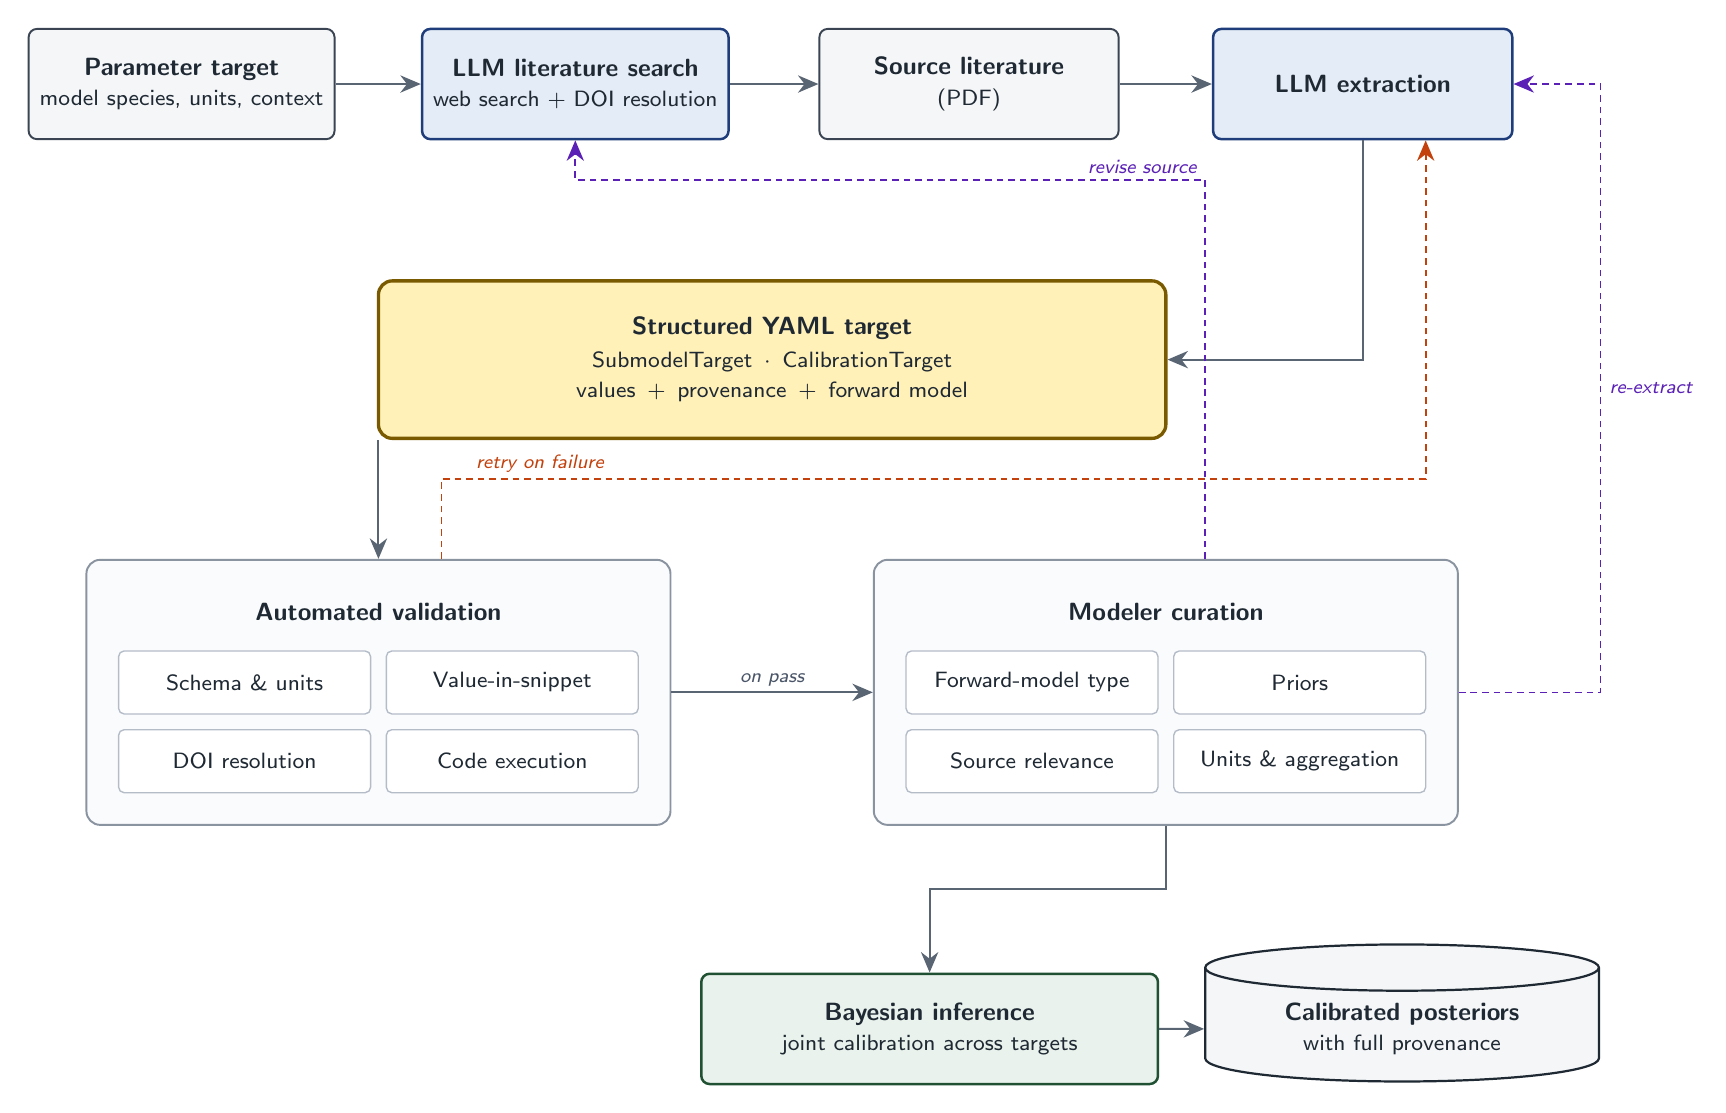
\begin{tikzpicture}[x=1mm, y=1mm]

% ============================================
% Coordinate system (mm): x in [0,200], y inverted (top-down)
% Row 1 (input chain):   y = 120
% Row 2 (YAML hub):      y =  85
% Row 3 (validate/curate): y =  40
% Row 4 (inference/post): y =   0
% ============================================

% ----- Row 1: input chain at y=120 -----
\node[stage] (target)  at ( 25,120) {Parameter target\\\footnotesize\mdseries model species, units, context};
\node[llm]   (search)  at ( 75,120) {LLM literature search\\\footnotesize\mdseries web search + DOI resolution};
\node[stage] (src)     at (125,120) {Source literature\\\footnotesize\mdseries (PDF)};
\node[llm]   (extract) at (175,120) {LLM extraction};

% ----- Row 2: YAML hub at y=85 -----
\node[hub] (yaml) at (100,85) {%
  Structured YAML target\\[1pt]
  \footnotesize\mdseries SubmodelTarget \,$\cdot$\, CalibrationTarget\\
  \footnotesize\mdseries values \,+\, provenance \,+\, forward model%
};

% ----- Row 3: Validation (left) and Curation (right) at y=40 -----
% Validation chips, 2x2 grid centered at x=50, y=40
\node[chip] (vschema)  at ( 33, 44) {Schema \& units};
\node[chip] (vsnippet) at ( 67, 44) {Value-in-snippet};
\node[chip] (vdoi)     at ( 33, 34) {DOI resolution};
\node[chip] (vcode)    at ( 67, 34) {Code execution};

\node[grouplabel] (vlabel) at (50, 53) {Automated validation};

\begin{scope}[on background layer]
  \node[groupbg, fit=(vlabel)(vschema)(vsnippet)(vdoi)(vcode)] (validate) {};
\end{scope}

% Curation chips, 2x2 grid centered at x=150, y=40
\node[chip] (cfm)      at (133, 44) {Forward-model type};
\node[chip] (cpriors)  at (167, 44) {Priors};
\node[chip] (crel)     at (133, 34) {Source relevance};
\node[chip] (cunits)   at (167, 34) {Units \& aggregation};

\node[grouplabel] (clabel) at (150, 53) {Modeler curation};

\begin{scope}[on background layer]
  \node[groupbg, fit=(clabel)(cfm)(cpriors)(crel)(cunits)] (curate) {};
\end{scope}

% ----- Row 4: Inference (below curate) and Posteriors at y=0 -----
\node[infer]   (infer) at (120, 0) {Bayesian inference\\\footnotesize\mdseries joint calibration across targets};
\node[outnode] (post)  at (180, 0) {Calibrated posteriors\\\footnotesize\mdseries with full provenance};

% ============================================
% Forward edges
% ============================================
\draw[flow] (target)  -- (search);
\draw[flow] (search)  -- (src);
\draw[flow] (src)     -- (extract);

% Extract -> YAML (single arrow from middle-top)
\draw[flow] (extract.south) |- ($(yaml.east) + (8,0)$) -- (yaml.east);

% YAML -> Validate
\draw[flow] (yaml.south -| validate.north) -- (validate.north);
% Validate -> Curate
\draw[flow] (validate.east) -- node[edgelabel, above]{on pass} (curate.west);
% Curate -> Inference: down, then left, then down again into infer.north
% (avoids running along the top edge of the inference box).
\draw[flow] (curate.south) -- ++(0, -8) -| (infer.north);
% Inference -> Posteriors
\draw[flow] (infer) -- (post);

% ============================================
% Feedback (back) edges — orthogonal routes that go AROUND the hub.
% Hub spans roughly x=[50,150], y=[75,95]. Gap below hub: y in [55,75].
% Gap above hub (between hub and row 1): y in [95,113].
% ============================================

% retry on failure (validate -> extract): goes BELOW hub then up around its
% RIGHT side. Source nudged east of validate.north, landing nudged east of
% extract.south.
\draw[back] ($(validate.north) + (8, 0)$)
  |- node[backlabel, pos=0.55, above]{retry on failure}
     ($(extract.south) + (8, -43)$)
  -- ($(extract.south) + (8, 0)$);

% revise source (curate -> search): goes ABOVE hub. |- forces a perfect
% vertical-then-horizontal corner at the bend.
\draw[modelerback] ($(curate.north) + (5, 0)$)
  |- node[modelerlabel, pos=0.55, above]{revise source}
     ($(search.south) + (0, -5)$)
  -- (search.south);

% curate -> extract  (re-extract)
\draw[modelerback] (curate.east) -- ++(18,0)
  |- node[modelerlabel, pos=0.25, right=1pt]{re-extract}
  ($(extract.east) + (6,0)$) -- (extract.east);


\end{tikzpicture}
\end{document}
